\documentclass[a4,paper,fleqn]{article}

\usepackage{layout}

\newcommand{\uuline}[1]{{\underline{\underline{#1}}}}

\title{AES - Übung 6 \\Auslegung einer netzgekoppelten PV-Anlage}
\date{\today}
\author{Daniel Winz}

\begin{document}
\maketitle
%\clearpage
\vfill
\tableofcontents
\vfill
\clearpage

\section{Ausgangslage}
Es ist eine Photovoltaikanlage für ein Flachdach ausgelegt werden. Dabei ist 
sowohl der Energieertrag als auch die Kosten berücksichtigt werden. 

\begin{figure}[h!]
    \centering
    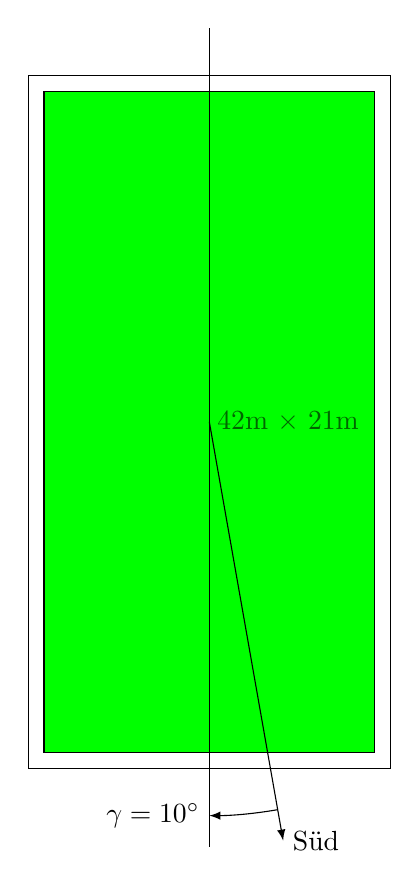
\begin{tikzpicture}[scale=2]
        \draw[] (-1.15,-2.2) rectangle (1.15,2.2);
        \draw[fill=green] (-1.05,-2.1) rectangle (1.05,2.1);
        \draw (0,2.5) -- (0,-2.7);
        \draw[-latex] (0,0) -- (280:2.7) node[right] {Süd};
        \draw[latex-] (0,-2.5) node[left] {$\gamma = 10^\circ$} 
            arc [start angle=270, end angle=280, radius=2.5];
        \node[green!40!black] at (0.5,0) {42m $\times$ 21m};
    \end{tikzpicture}
    \label{fig:roof}
    \caption{Geometrie und Ausrichtung des Flachdachs}
\end{figure}

\clearpage
\begin{appendix}
\section{Daten Solarpanels}
\begin{zebratabular}{lllll}
\rowcolor{gray}
Solarmodul &
    PV\_A &
    PV\_B &
    PV\_C &
    PV\_D \\
Aufbau &
    Polykristallin &
    Monokristallin &
    Monokristallin &
    Monokristallin \\
Herkunft &
    CH &
    CH &
    China &
    Japan \\
$P_G$ $[W_p]$ &
    240 &
    245 &
    260 &
    240 \\
Masse $[mm]$ &
    992 $\times$ 1650 x 45 &
    991 $\times$ 1656 x 65 &
    992 $\times$ 1636 x 45 &
    798 $\times$ 1580 x 35 \\
$U_{mpp}$ $[V]$ &
    30 &
    30.2 &
    30.6 &
    43.7 \\
$U_{OC}$ $[V]$ &
    37.2 &
    36.9 &
    37.3 &
    52.4 \\
$\Delta U_{OC}$ $[\%/^\circ C]$ &
    -0.33 &
    -0.36 &
    -0.31 &
    -0.25 \\
$I_{mpp}$ $[A]$ &
    8 &
    8.1 &
    8.5 &
    5.51 \\
$I_{SC}$ $[A]$ &
    8.65 &
    8.6 &
    9.18 &
    5.85 \\
$\eta$ $[\%]$ &
    14.7 &
    14.9 &
    16 &
    19 \\
Preis $[CHF]$ &
    242 &
    333 &
    224 &
    589 \\
\end{zebratabular}

\section{Daten Wechselrichter}
\begin{zebratabular}{lllll}
\rowcolor{gray}
Solarmodul &
    WR\_A &
    WR\_B &
    WR\_C &
    WR\_D \\
Beschreibung &
    Zentral-WR gross &
    Zentral-WR klein &
    Multistring WR 2 Strings &
    Multistring WR 3 Strings \\
$P_W$ $[kW]$ &
    80 &
    35 &
    10 &
    15 \\
$P_{G_{max}}$ pro String $[kW]$ &
    k. A. &
    k. A. &
    9 &
    9 \\
$U_{min}$ für $P_W$ $[V]$ &
    k. A. (430?) &
    k. A. (400?) &
    290 &
    320 \\
$U_{MPP}$ Bereich $[V]$ &
    430 \ldots 800 &
    400 \ldots 800 &
    250 \ldots 750 &
    250 \ldots 750 \\
$U_{OC_{max}}$ $[V]$ &
    900 &
    900 &
    900 &
    900 \\
$I_{W_{max}}$ $[A]$ &
    180 &
    78 &
    18 &
    16 \\
$\eta_{WR}$ $[\%]$ &
    95.5 &
    96.1 &
    97.5 &
    97.5 \\
Preis $[CHF]$ &
    28'910 &
    11'392 &
    3'366 &
    4'248 \\
\end{zebratabular}

\section{Daten Anschlusskasten}
\begin{zebratabular}{llll}
\rowcolor{gray}
Anschlusskasten &
    AK\_1 &
    AK\_2 &
    AK\_3 \\
Art &
    DC, 16 $\to$ 1 &
    DC, 12 $\to$ 1 &
    AC, 3 phasig \\
Preis $[CHF]$ &
    2'530 &
    2'156 &
    1'000 \\
\end{zebratabular}

\clearpage
\section{Matlab Funktion panelize.m}
\label{app_panelize}
\lstsettingmatlab
\lstinputlisting{panelize.m}

\clearpage
\section{Matlab Skript panels.m}
\label{app_panels}
\lstsettingmatlab
\lstinputlisting{panels.m}

\end{appendix}
\end{document}
